%%
\label{chap-WAD}


Here some properties of the algorithm given in \secref{mdsdist} are given.

\section{Preliminaries}

To begin with some preliminaries. Notation is as in \secref{mdsdist}, but is refreshed here. In this section a proof of the uniqueness of the shortest path in a simple polygon is given.

\subsection{Notation}

DEFINE everything here: COMBINE!

$p_1$ and $p_2$ always refer to the two points that we want to find the shortest path between

$\Gamma$ is the polygon that we are interested in

$v_i$ refers to a point in a path within the domain, it may or may not be a vertex of $\Gamma$.

$\mathcal{P}_1$ and $\mathcal{P}_2$ are the initial paths between $p_1$ and $p_2$ that trace the boundary.

$\mathcal{P}$ is the working path between $p_1$ and $p_2$.


$\mathcal{S}_{i}$ is a section of a path.

\subsection{Terminology}

The word triangle here is used to refer to the case in which three points, $(v_i,v_{i+1},v_{i+2})$ are vertices of a triangle all the adges of which lie within $\Gamma$. These are the cases in which the DELETE would simplify $(v_i,v_{i+1},v_{i+2})$ to $(v_i,v_{i+2})$.


\subsection{Uniqueness of shortest path}
\label{app-unique-sp}
Propostition: there is one, unique shortest path between point $p_1$ and $p_2$ within a simple polygon (ie. the polygon has no holes), $\Gamma$.

This is simple to see since if the shortest path were non-unique then there would exist $\mathcal{P}_A$ and  $\mathcal{P}_B$ which were both shortest paths between $p_1$ and $p_2$. It would then be the case there there would be two points $v_1^*$ and $v_2^*$ say where the paths started to differ and ended differing (these could be $p_1$ and $p_2$): the points at which $\mathcal{P}_A$ and  $\mathcal{P}_B$ become disjoint. Call the two paths that lie between $v_1^*$ and $v_2^*$ $\mathcal{S}_{AB}$ and $\mathcal{S}_{BA}$. 

Joining up $\mathcal{S}_{AB}$ and $\mathcal{S}_{BA}$ at $v_1^*$ and $v_2^*$ forms a loop, $\mathcal{L}$, say. There is nothing in the middle of $\mathcal{L}$ (since $\Gamma$ has no holes), in which case there must be a kink in at least one of the paths (since they are not identical, at least one of them must not be a straight line between $v_1^*$ and $v_2^*$), this means that there is a triangle in (at least) one of the paths, which can be straightened ($\mathcal{L}$ does not contain any obstacle stopping this) so the path is not a shortest path and can be shortened. This is a contradiction, therefore the shortest path must be unique. Figure \ref{app-WAD-unique-dia} may be helpful.

This proof was adapted from the one given in lecture notes by Leonidas Guibas available at \url{http://graphics.stanford.edu/courses/cs268-09-winter/}.


\begin{figure}
\centering
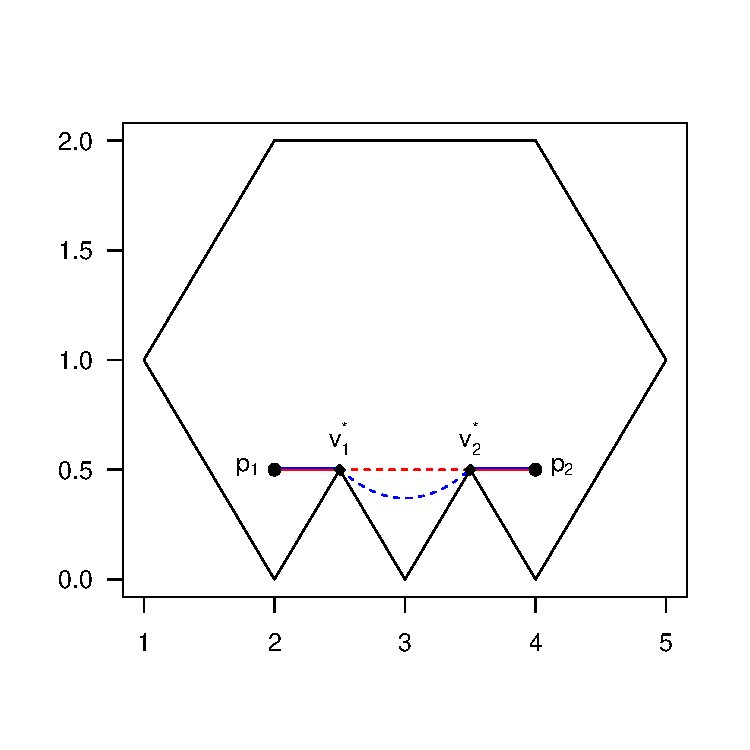
\includegraphics[width=3in]{app-WAD/figs/unique-path-dia.pdf} \\
\caption{Illustration of some of the terms used in the proof that there is always a unique shortest path. $\mathcal{P}_A$ and  $\mathcal{P}_B$ are given by the red and blue lines. The loop ($\mathcal{L}$) is given by the dotted lines; the red part is  $\mathcal{S}_{AB}$ and the blue part  $\mathcal{S}_{BA}$.}
\label{app-WAD-unique-dia}
% generated by thesis/app-WAD/figs/unique-shortest-path.R
\end{figure}



\section{Properties}

\subsection{The algorithm terminates}

The condition to be fulfilled for the algorithm to terminate is that in two consecutive runs the path does not change, so the first step is to check that it is possible for this to happen, then to move on to show that it always happens. 

First note that the ALTER step can act as (a less efficient) DELETE step: $\mathcal{P}_{I}$ would be the triplet $(v_i,v_{i+1},v_{i+2})$ (a triangle) then the DELETE substep removes $v_{i+1}$, giving $(v_i,v_{i+2})$), which would then be $\mathcal{P}_{ID}$ which could be inserted into the path. For this reason we only need to consider the ALTER step here.


THIS IS WRONG

Some triplet effects the path of another. Show that local optimality -> global optimality.

First show that ALTER is locally optimal

DELETE case is obvious.

THINK about convex/concave

paths always get shorter


For the algorithm to fail to terminate, the situation would have to arise in which one ALTER step would take the path $\mathcal{P}_1^*$ (say) and alter it to be $\mathcal{P}_2^*$ such that the next ALTER step would revert $\mathcal{P}_2^*$ back to $\mathcal{P}_1^*$, these two steps would then continue indefinitely.

If this were to happen it would imply that both $\mathcal{P}_2^*$ was shorter than $\mathcal{P}_1^*$ and $\mathcal{P}_1^*$ was shorter than $\mathcal{P}_2^*$ and since in the ALTER step the $\mathcal{P}_{ID}$ must be shorter than $(v_i,v_{i+1},v_{i+2})$ (not equal in length) then this cannot happen.

Clearly the algorithm cannot continue shortening the path forever, at some point there will be no more shorter routes proposed by the ALTER step and hence it will terminate.


\subsection{The algorithm terminates at the shortest path}

Consider the two initial paths following the boundary, $\mathcal{P}_1$ or $\mathcal{P}_2$ above. Without loss of generality, let $\mathcal{P}_1$ be the shorter of the two initial paths. The DELETE and ALTER steps can be thought of as refining $\mathcal{P}_1$ of these starting paths.

We can think of $\mathcal{P}_1$ as traversing a series of features of the boundary and we would like to include as few of them as possible to obtain the shortest path. The features fall into two classes, they are concave and convex. The names are given as they would appear to one traversing them from inside the domain, so they appear to be opposite to the definitions as used to describe polygons. Concave features extrude from the polygon (ie. they would look like ``caves'' to those traversing the boundary) and convex features intrude into the polygon (ie. they would look like ``mountains'' to those traversing the boundary).




Concave features consist of a set of vertices $(v_i, v_{i+1},\cdots,v_{i+k})$, where all of the vertices between $v_i$ and $v_{i+k}$ can be removed without any of the path falling outside of the domain, one can think of this as capping the top of a cave.

Convex features consist of a series of vertices where only some of the 


The shortest path through a concave section can always be found in a series of DELETE steps: if the concave section alone is taken and triangulated, the DELETE step will always be able to remove all of the vertices in the concave section (since it can be triangulated). This leaves only the starting and ending vertices. Figure \ref{app-WAD-concave} shows how the triangulation removes the vertices.


TKTKTK diagram

Having removed all of the concave parts of the path, this leaves only convex features. In order to find the shortest path around them we can simply trace them (they cannot be reduced any further since they are already convex). It might then be the case that by tracing these convex features further convex and concave features are introduced, however these can be addressed in the next iteration.

The only thing it remains to consider is the points at which the convex segment joins the rest of the path, these may be shortened by using the DELETE step if necessary.

Given that the initial path many consist of only these two elements and that they are removed by the consecutive steps of DELETE and ALTER (obviously there may need to be micro steps of these within each step due to the aforementioned embeddding of caves-within-mountains and mountains-within-caves) we can conclude that the path is the shortest path.

CAN WE?!?!?!?!?!

\subsection{The computational complexity of the algorithm}





